\chapter{Annex}\label{sec:irgendwas}

\section{Segmentation Frequency}
\label{subsec:segmentation-frequency}

The process of segmenting point clouds is one of the more computationally intensive parts of the pipeline. This motivates the development of a well-designed segmentation strategy - that is, a process driving the decision of which areas of the local cloud to segment, and when.\\

Regarding time: it is intuited that regions of space should be passed through the segmenter when they are most accurate and dense. This presents a trade-off problem. The longer one waits before segmenting, the worse positioning confidence is, and the larger the uncertainty in the points' fixed frame position (this leads to 'fuzzy' segments).
Not waiting long enough, on the other hand, leads to sparse segments, which might be missing important geometrical information, or introduce artefacts - such as scan-line patterns.
One way of handling this trade-off is to set a `sufficient density', where it is estimated that increasing density leads to diminishing information gain. 
From that point on, the costs of increasing density - i.e. loss of accuracy - outweigh the benefits, and segmentation should be undertaken. We determine this 'sufficient density' empirically and qualitatively, through visual analysis of the accumulated map at various points in time.\\

During the process of accumulating a local map, regions at different distances from the sensor densify at different rates. Thus various regions will reach sufficient density at different times.
Within this paradigm, it would be optimal to segment different areas at different times even though they were captured simultaneously.
This would lead to quite complicated algorithms, and increase the amount of parameters which need to be tuned.\\

However, though far away objects densify more slowly, they accumulate positional uncertainty faster. They are also less useful for positioning and place recognition, due to parallax effects.
Thus it can be advantageous to prioritize closer objects, which allows one to assume a single rate of density increase for the whole area being captured - fixed to the close objects densification rate.\\

The resulting strategy is excessively simple: accumulate all points, until target density is reached in nearby objects, then segment all accumulated points. After segmentation, discard those points and start over. Thus only a single approximate rate of densification is considered.\\

A further idealization is to relate this densification rate to movement. This is particularly true of rotating LIDAR systems such as the velodyne, with which the sensor can only cover new areas if the robot moves.  
According to this idealization, when the robot has travelled a certain distance $\Delta x$ nearby segments densify by a certain amount $\Delta D$, and the relationship between the two is modelled with a simple proportionality,
$$\frac{\Delta x}{\Delta D} = \alpha$$
Where alpha is assumed to be an unknown constant. With this assumption, we are able to conclude that target density is reached when
$$x_{target} = D_{target} * \alpha$$
which gives us a simple rule: Segment the cloud every time the robot has moved/rotated by a certain amount $x_{target}$. Through experiments, we determine that an acceptable value for $x_{target}$ is 20 meters.\\

This affords a relatively simple implementation, with the added advantage that it makes relating segments to poses straightforward.\\



\section{Latent Space Dimension}
\label{sec:latent_space_size}

In the process of selecting the autoencoder architecture, a comparison was made between sizes in the latent space. The goal was to encode the segment descriptions with as small a dimensionality as possible, in order to show that the autoencoder could perform better than other descriptors even for similar description sizes. Another advantage of keeping descriptions small is that they would require less storage space when running SegMatch on long datasets.\\

Non-trivial improvements in reconstruction quality were observed when switching from a latent space size of 10 to 15. However, larger dimensionalities showed increased redundancies in the latent space (such as unused dimensions, discussed in Chapter \ref{chap:ae}, Section \ref{sec:ae-results}, or lack of insignificant improvements in reconstruction ability).\\

As an extremum example, a model with a 2-dimensional latent space was trained similarly to the regular models. The distribution of segment descriptions in this 2D space is shown in Fig.~\ref{fig:2d_latent_space}. The model's reconstruction abilities were observed as quite limited, often failing to produce a reconstruction, or reconstructing segments of a certain class as 3D clusters resembling segments of an entirely different class. In accordance with this, there is much overlap between classes visible in Fig.~\ref{fig:2d_latent_space}.\\

\begin{figure}
  \centering
  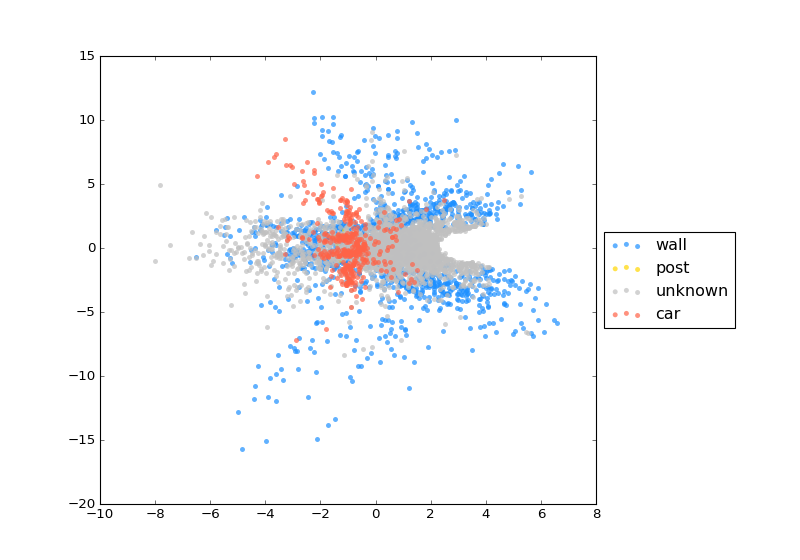
\includegraphics[width=5.2in]{images/2dlatentspace.png}
  \caption{Segment descriptions given by a 2-dimensional latent space autoencoder model}
  \label{fig:2d_latent_space}
\end{figure}

